My various attention-based models are classifed into two broad categories, {\it global} and {\it local}. These classes differ in terms of whether the ``attention'' is placed on all source positions or on only a few source positions. I illustrate these two model types in Figure~\ref{f:soft_attn} and \ref{f:hard_attn} respectively.

Common to these two types of models is the fact that at each time step $t$ in the decoding phase, both approaches first take as input the hidden state $\hi$ at the top layer of a stacking LSTM. The goal is then to derive a context vector $\co$ that captures relevant source-side information to help predict the current target word $\tgt{t}$. While these models differ in how the context vector $\co$ is derived, they share the same subsequent steps. 

Specifically, given the target hidden state $\hi$ and the source-side context vector $\co$, I employ a simple concatenation layer to combine the information from both vectors to produce an attentional hidden state as follows:
\begin{equation}
\hs = \tanh(\W{c}[\co; \hi])
\label{e:hs}
\end{equation} 

The attentional vector $\hs$ is then fed through the softmax layer to produce the predictive distribution formulated as:
\begin{equation}
p(\tgt{t}|\tgt{<t},\src{}) = \softmax(\W{s}\hs)
\label{e:predict}
\end{equation} 

I now detail how each model type computes the source-side context vector $\co$.

\subsection{Global Attention}
\label{subsec:global}
\begin{figure}
\centering
%\psgrid
\rput(6.3,6.2){$\tgt{t}$}
\rput(6.6,5.7){$\hs$}
\rput(2.2,3.5){$\co$}
\rput(4.3,2.5){$\al$}
\rput(6.75,1.7){$\hi$}
\rput(0.2,2.1){$\his$}
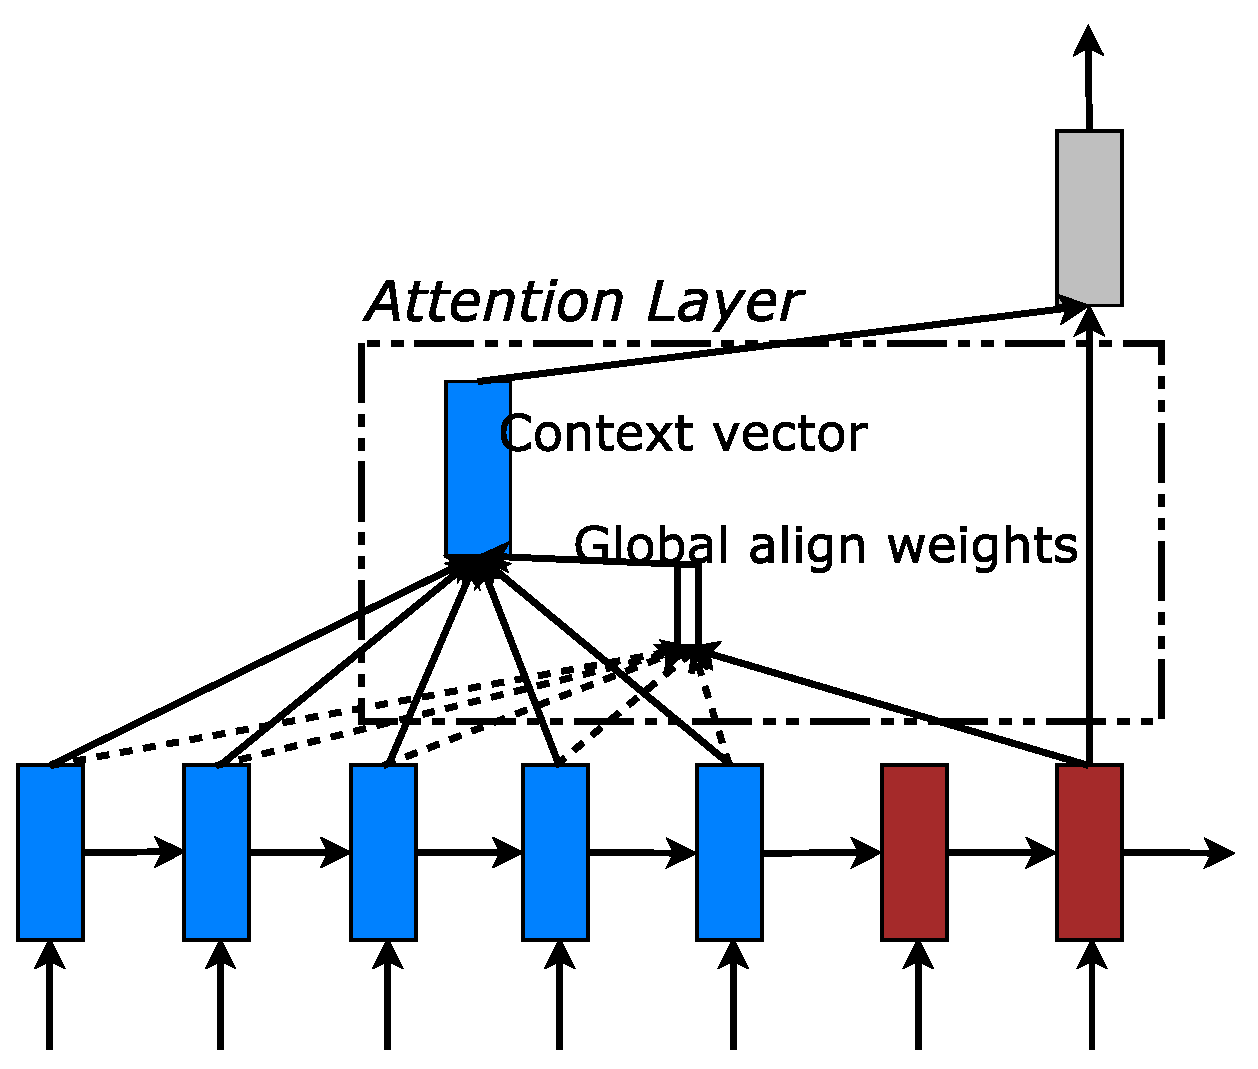
\includegraphics[width=0.45\textwidth, clip=true, trim= 0 0 0 0]{img/4-attn_soft} % , angle=-90
\caption[Global attentional model]{{\bf Global attentional model} -- at each time step $t$, the model infers a {\it variable-length} alignment weight vector $\al$ based on the current target state $\hi$ and all source states $\his$. A global context vector $\co$ is then computed as the weighted average, according to $\al$, over all the source states. 
} 
\label{f:soft_attn}
\end{figure}

The idea of a global attentional model is to consider all the hidden states of
the encoder when deriving the context vector $c_t$. In this model type, a
variable-length alignment vector $\al$, whose size equals the number of time
steps on the source side, is derived by comparing the current target hidden
state $\hi$ with each source hidden state $\his$:
\begin{align}
\label{e:al}
\al(s)&=\alignf(\hi, \his) \\
&=\frac{\exp \open{\score(\hi, \his)}}{\sum_{s'} \exp \open{\score(\hi,
\MB{\bar{h}}_{s'})}} \notag
\end{align}
Here, $\score$ is referred as a {\it content-based} function for which I consider three different
alternatives:
\begin{equation*}
\score(\hi, \his)\!=\!\begin{cases}
    \tp{\hi} \his & \mbox{{\it dot}}\\
    \tp{\hi} \MB{W_a} \his & \mbox{{\it general}} \\
    \tp{\MB{v}_a}\tanh\open{\MB{W_a} [\hi; \his]} & \mbox{{\it concat}}
\end{cases}
\end{equation*}

Besides, in our early attempts to build attention-based models, I use
a {\it location-based} function in which the alignment scores are
computed from solely the target hidden state $\hi$ as
follows:
\begin{equation}
\al = \softmax(\W{a}\hi) \mbox{ } \mbox{ } \mbox{ } \mbox{ } \mbox{ } \mbox{ } \mbox{ } \mbox{ } \mbox{ } \mbox{ } \mbox{ } \mbox{ } \mbox{ } \mbox{ } \mbox{ } \mbox{ } \mbox{{\it location}}
\label{e:location}
\end{equation}
Given the alignment vector as weights, the
context vector $c_t$ is computed as the  weighted average over all the source hidden states.\footnote{\eq{e:location} implies that
all alignment vectors $\al$ are of the same length. For short sentences, I only
use the top part of $\al$ and for long sentences, I ignore words near the end.}

\textit{Comparison to \cite{bog15}} --
% An example of such model is the work of \newcite{bog15}. 
While our global attention approach is similar in spirit to the model proposed
by \newcite{bog15}, there are several key differences which reflect how I have
both simplified and generalized from the original model. First, I simply use
hidden states at the top LSTM layers in both the encoder and decoder as
illustrated in Figure~\ref{f:soft_attn}. \newcite{bog15}, on the other hand,
use the concatenation of the forward and backward source 
hidden states in the bi-directional encoder and target hidden
states in their non-stacking uni-directional decoder. Second, our computation
path is simpler; I go from $\hi \rightarrow \al \rightarrow \co \rightarrow
\hs$ then make a prediction as detailed in \eq{e:hs}, \eq{e:predict}, and
Figure~\ref{f:soft_attn}. On the other hand, at any time $t$, \newcite{bog15} build from the previous hidden state $\hid{t-1} \rightarrow \al \rightarrow \co \rightarrow \hi$, which, in turn, goes through a deep-output and a maxout layer before making predictions.\footnote{I will refer to this difference again in Section~\ref{subsec:input}.} Lastly, \newcite{bog15} only experimented with one alignment function, the {\it concat} product; whereas I show later that the other alternatives are better.

\subsection{Local Attention}
\begin{figure}
\centering
%\psgrid
\rput(6.3,6.2){$\tgt{t}$}
\rput(6.6,5.7){$\hs$}
\rput(2.2,3.5){$\co$}
\rput(3.0,2.4){$\al$}
\rput(6.75,1.7){$\hi$}
\rput(5.5,2.8){$p_t$}
\rput(0.2,2.1){$\his$}
%\rput(2.55,1.8){$p_t$}
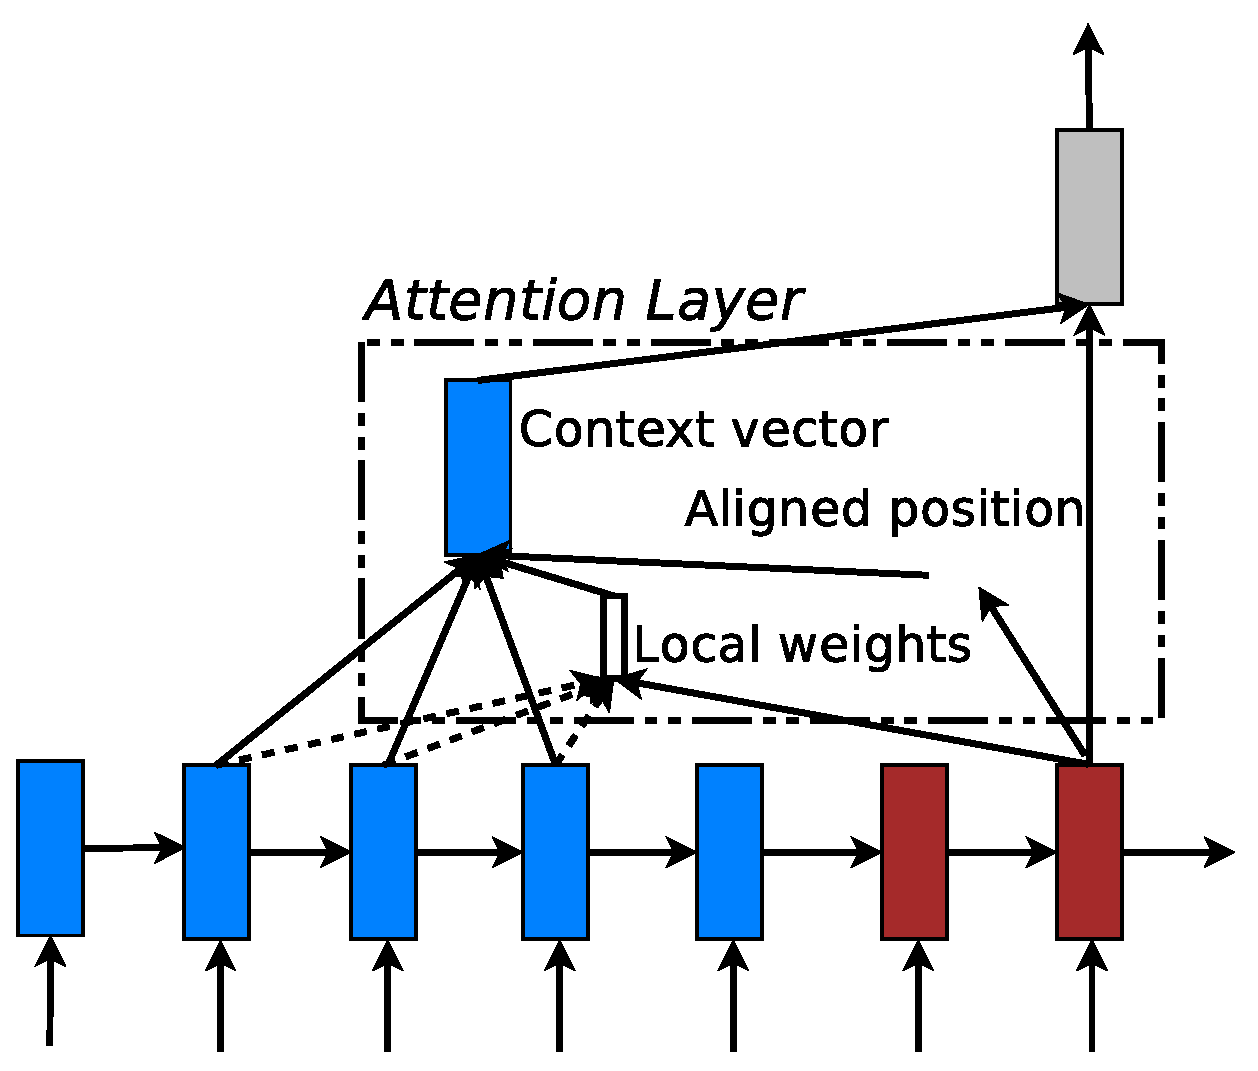
\includegraphics[width=0.45\textwidth, clip=true, trim= 0 0 0 0]{img/4-attn_hard} % , angle=-90
\caption[Local attention model]{{\bf Local attention model} -- the model first predicts a single
aligned position $p_t$ for the current target word. A window centered around the
source position $p_t$ is then used to compute a context vector $\co$, a weighted
average of the source hidden states in the window. The weights $\MB{\al}$ are
inferred from the current target state $\hi$ and those source states $\his$ in
the window.
%similar to the global attention model in Figure~\ref{f:soft_attn}, instead of producing a global alignment vector, 
} 
\label{f:hard_attn}
\end{figure}

The global attention has a drawback that it has to attend to all words on the
source side for each target word, which is expensive and can potentially render it impractical to
translate longer sequences, e.g., paragraphs or documents.
To address this deficiency, I propose a {\it local} attentional mechanism that
chooses to focus only on a small subset of the source positions per target word.

This model takes inspiration from the tradeoff between the {\it soft} and {\it
hard} attentional models proposed by \newcite{xu15} to tackle the image caption
generation task. In their work, soft attention refers to the global attention
approach in which weights are placed ``softly'' over all patches in the source
image. The hard attention, on the other hand, selects one patch
of the image to attend to at a time. While less expensive at inference time, the
hard attention model is non-differentiable and requires more complicated
techniques such as variance reduction or reinforcement learning to train.

Our local attention mechanism selectively focuses on a small window of
context and is differentiable. This approach has an advantage of avoiding the expensive computation incurred in
the soft attention and at the same time, is easier to train than the hard
attention approach.
In concrete details, the model first generates an aligned position $p_t$ for each target word at time $t$. The
context vector $\co$ is then derived as a weighted average over the set of source hidden states within the window $[p_t-D, p_t+D]$; $D$ is
empirically selected.\footnote{If the window crosses the sentence boundaries, I
simply ignore the outside part and consider words in the window.} Unlike the global approach, the local alignment vector $\al$ is now fixed-dimensional, i.e., $\inR{2D+1}$. %is generated in the same manner as the global attentional model except that its dimension is $(2D+1)$.
I consider two variants of the model as below.

\textit{Monotonic} alignment ({\bf \localm{}}) -- I simply set % 
$\pt\!=\!t$ assuming that source and target sequences are roughly
monotonically aligned. The alignment vector $\al$ is defined according to
\eq{e:al}.\footnote{{\it local-m} is the same as
the global model except that the vector $\al$ is
fixed-length and shorter.} % This model is differentiable.

\textit{Predictive} alignment ({\bf \localp{}}) --  %
instead of assuming monotonic alignments, our model predicts an aligned position as follows:
\begin{equation}
\pt = S \cdot \sigmoid(\tp{\MB{v}_p}\tanh(\W{p}\hi)),
\label{e:p}
\end{equation}
$\W{p}$ and $\MB{v}_p$ are the model parameters which will be learned
to predict positions. $S$ is the source sentence length. As a result of $\sigmoid$, $\pt
\in [0, S]$. To favor alignment points near $\pt$, I place a Gaussian distribution centered around $\pt$ . Specifically, our alignment weights are now
defined as:
\begin{equation}
\al(s) = \alignf(\hi, \his) \exp \open{-\frac{(s-\pt)^2}{2\sigma^2}} 
\label{e:align_p}
\end{equation}
I use the same $\alignf$ function as in
\eq{e:al} and the standard deviation is empirically set as
$\sigma\!=\!\frac{D}{2}$. Note that $\pt$ is a {\it real} nummber; whereas $s$
is an {\it integer} within the window centered at $\pt$.\footnote{{\it local-p} is similar to the
local-m model except that I dynamically
compute $\pt$ and use a truncated Gaussian distribution to modify the original alignment
weights $\alignf(\hi, \his)$ as shown in \eq{e:align_p}. By utilizing $\pt$
to derive $\al$, I can compute backprop gradients for $\W{p}$ and $\MB{v}_p$.
This model is differentiable almost everywhere.} 

\textit{Comparison to \cite{draw15}} --
have proposed a {\it selective attention} mechanism, very
similar to our local attention, for the image generation task. Their approach 
allows the model to select an image patch of varying location and zoom. I,
instead, use the same ``zoom'' for all target positions, which greatly
simplifies the formulation and still achieves good
performance.

\subsection{Input-feeding Approach}
\label{subsec:input}
In our proposed global and local approaches, the attentional decisions are made
independently, which is suboptimal. Whereas, in standard MT, a {\it coverage}
set is often maintained during the translation process to keep track of which
source words have been translated. Likewise, in attentional NMTs, alignment
decisions should be made jointly taking into account past alignment information.
To address that, I propose an {\it input-feeding} approach in which attentional
vectors $\hs$ are concatenated with inputs at the next time steps as illustrated in
Figure~\ref{f:input}.\footnote{If $n$ is the number of LSTM cells, the
input size of the first LSTM layer is $2n$; those of subsequent
layers are $n$.} The effects of having such connections are two-fold:
(a) I hope to make the model fully aware of previous alignment choices and (b)
I create a very deep network spanning both horizontally and vertically.

\begin{figure}
\centering
%\psgrid
\rput(3,5.6){$\hs$}
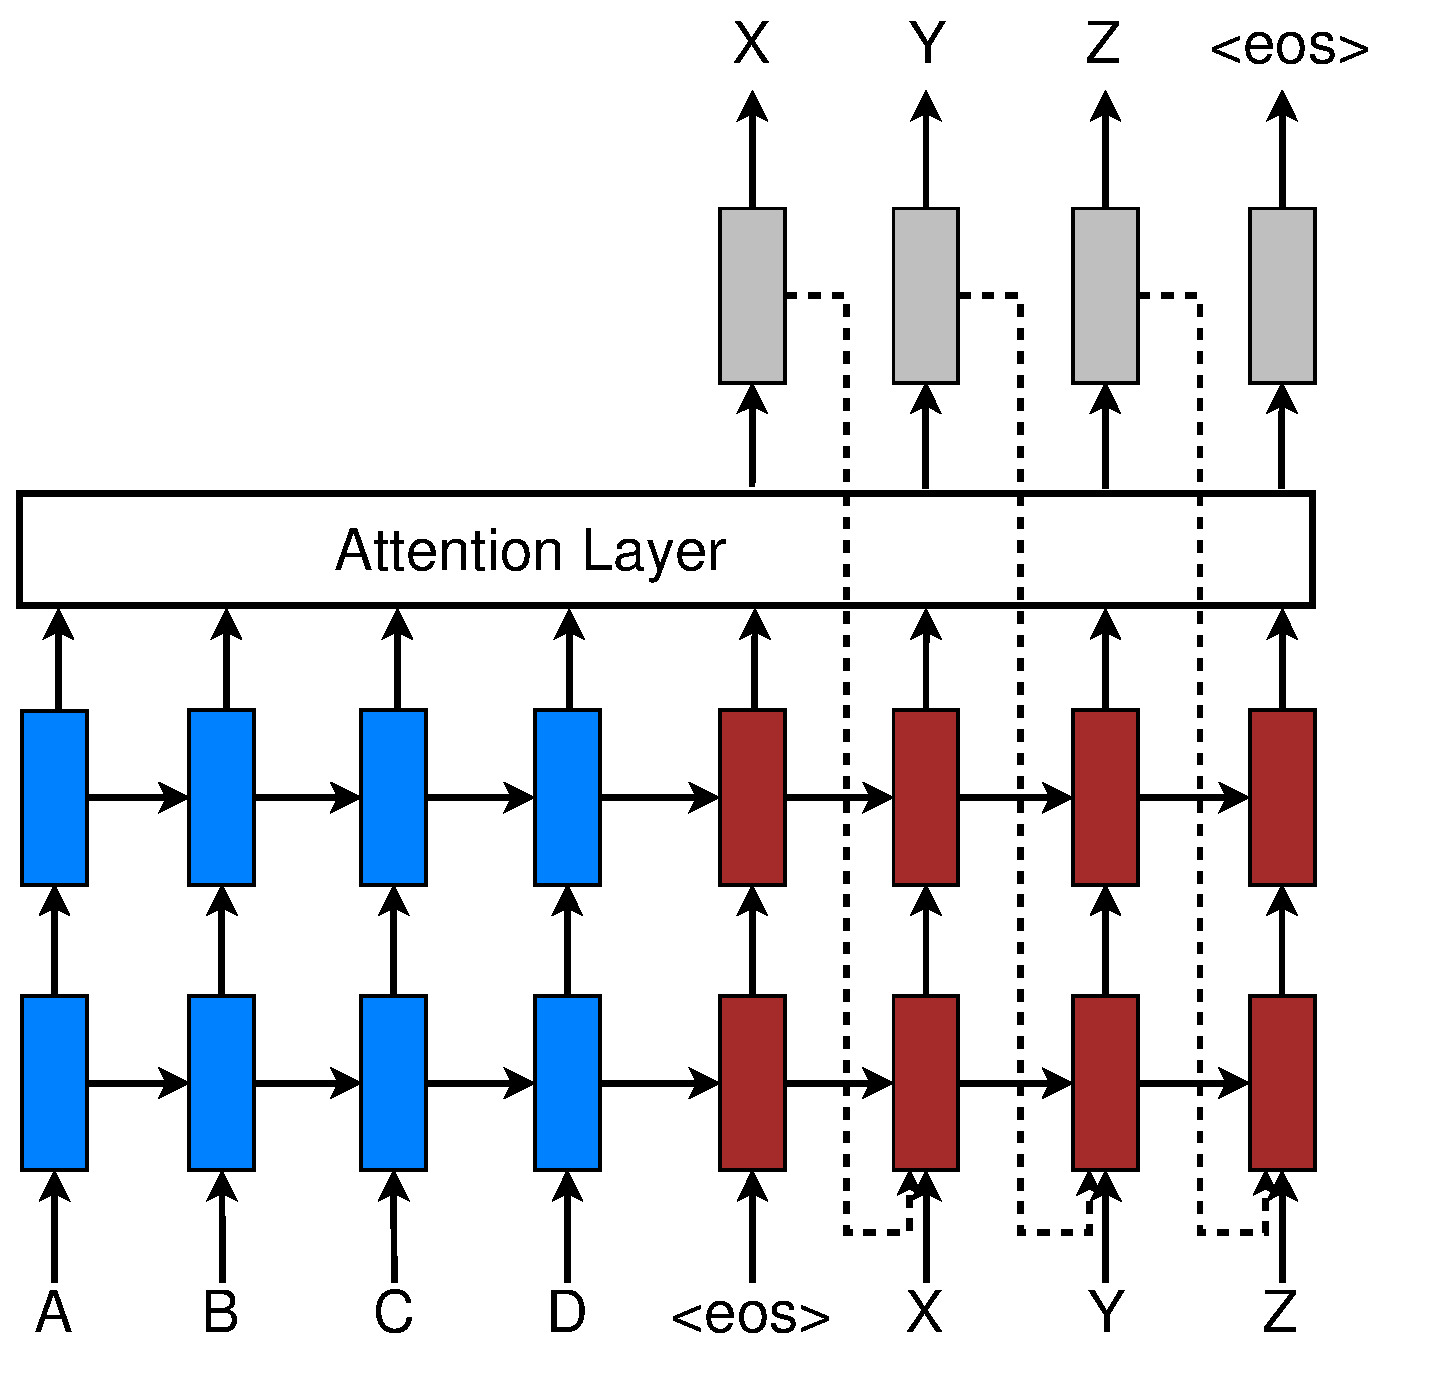
\includegraphics[width=0.4\textwidth, clip=true, trim= 0 0 0 0]{img/4-attn_input} % , angle=-90
\caption[Input-feeding approach]{{\bf Input-feeding approach} -- Attentional vectors $\hs$ are fed as inputs to the next time steps to inform the model about past alignment decisions.
} 
\label{f:input}
\end{figure}


{\it Comparison to other work} -- \newcite{bog15}
use context vectors, similar to
our $\co$, in building subsequent hidden states, which can also 
achieve the ``coverage'' effect. However, there has not been any analysis of 
whether such connections are useful as done in this work. Also,
our approach is more general; as illustrated in Figure~\ref{f:input}, it can be
applied to general stacking recurrent architectures, including non-attentional
models.

\newcite{xu15} propose a {\it doubly attentional} approach with an
additional constraint added to the training objective to make sure the model
pays equal attention to all parts of the image during the caption generation process. Such a constraint can also be useful to capture the coverage set effect in NMT that I mentioned earlier. However, I chose to use the input-feeding approach since it provides flexibility for the model to decide on any attentional constraints it deems suitable.
